\documentclass[a4paper]{article}
\usepackage{caption}
\usepackage{graphicx}
\usepackage[hidelinks]{hyperref}
\usepackage[dvipsnames]{xcolor}
\usepackage{url}
\usepackage{outlines}
\usepackage{listings}
\usepackage{fontspec}
\lstset{basicstyle=\ttfamily,
	showstringspaces=false,
	commentstyle=\color{blue},
	keywordstyle=\color{RubineRed}
}
\lstset{emph={
	EXPOSE,RUN,FROM,CMD,nc,tcp,udp,docker},emphstyle=\color{purple}
}
\newcommand{\abc}{\hfill \break}
\captionsetup{hypcap=true}
\usepackage{fancyhdr}
\usepackage{geometry}
\geometry{
	a4paper,
	total={170mm,257mm},
	left=20mm,
	top=20mm,
	bottom=39mm,
}

\setlength{\headheight}{82.70538pt}

\fancypagestyle{oida}{
	\fancyhf{}
	\fancyhead[L]{\fontsize{7.5}{7.5}htl donaustadt\\ Donaustadtstraße 45\\
		1220 Wien\\~\\ Abteilung: Informationstechnologie\\ 
	Schwerpunkt: Netzwerktechnik}
	\fancyhead[R]{
\includegraphics[scale=0.45]{images/logo.png}}

	\fancyfoot[L]{\today}
	\fancyfoot[C]{\jobname}
	\fancyfoot[R]{Page: \thepage}
}

\begin{document}
\bibliographystyle{IEEEtran}
\pagestyle{oida}
\section*{Ethical hacking of a CTF-VM}
\par\noindent\rule{\textwidth}{0.4pt}

Laboratory protocol
Exercise 7: Ethical hacking of a CTF-VM

\begin{figure}[h]
	
\includegraphics[scale=0.5]{images/menheraMagnifier.png}
	\centering
	\caption{Grouplogo}
\end{figure}

\vspace*{\fill}
Subject:	ITSI

Class:	3AHITN

Name:	Stefan Fürst, Justin Tremurici

Groupname/number Name here/12

Supervisor: 	SPAC, ZIVK

Exercise dates: 17-19.1.2025

Submission date: 20.1.2025


\newpage
\tableofcontents

\newpage

\section{Task definition}



\section{Summary}

\newpage

\section{Complete network topology of the exercise}
\begin{figure}[h]
	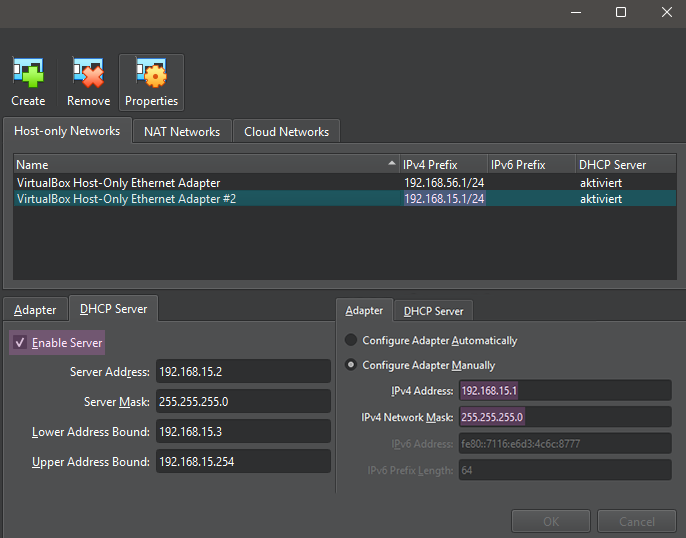
\includegraphics[scale=0.4]{./images/nwipsfr.png}
	\centering
	\caption{Complete network topology of the exercise}
\end{figure}\abc

\newpage

\section{Exercise Execution}
\subsection{Setting up the virtual machines.}
To get started with this CTF, make sure that VirtualBox version 7.1.4 is used. The VM to attack must be imported by double-clicking the provided \texttt{.ova} file. After the import is complete, the network settings must be changed to use Host-only Adapter mode. Since using the default Host-only network did not work, we had to create a new Host-only network. To do this, either press \texttt{<C-h>} or click on \texttt{File} > \texttt{Tools} > \texttt{Network Manager}, as shown in Figure 3.
\begin{figure}[h]
	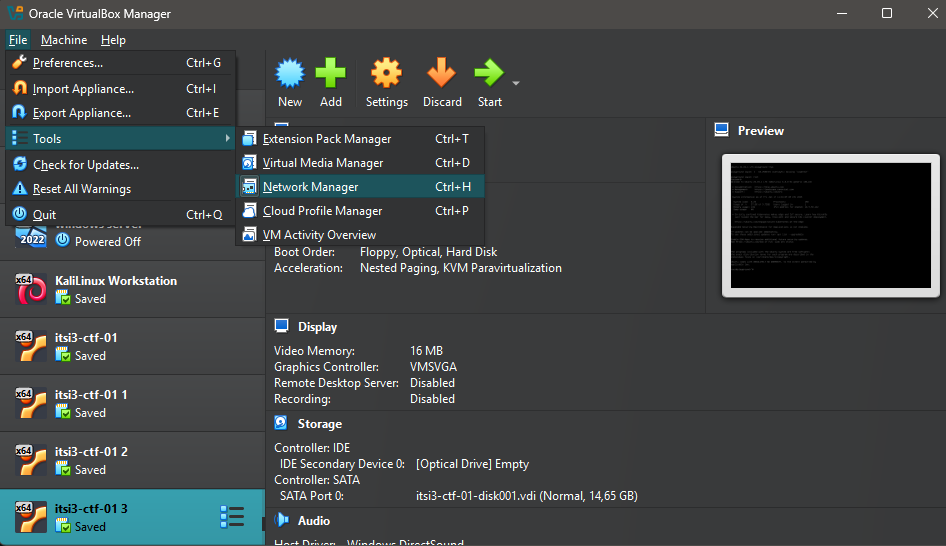
\includegraphics[scale=0.285]{./images/openingNetworkManager.png}
	\centering
	\caption{Opening VirtualBox Network Manager settings}
\end{figure}\abc
In this menu, click on \texttt{Create}, then check the \texttt{Enable Server} box to enable the DHCP server so the target VM will receive an IP address. Then, click on \texttt{Adapter} to view the IP range of the network, which in our case is \texttt{192.168.15.0/24}, which can be seen in Figure 4.
\begin{figure}[h]
	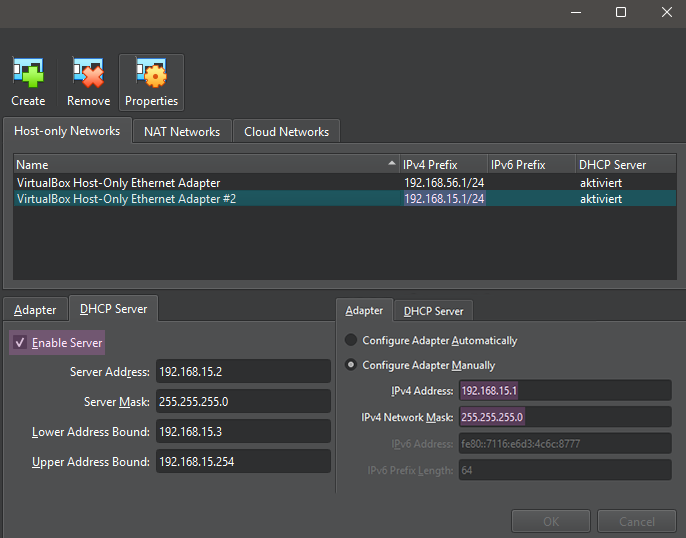
\includegraphics[scale=0.4]{./images/nwipsfr.png}
	\centering
	\caption{Showing the IP settings for the new Host-only network}
	\label{fig:nwconf}
\end{figure}\abc
Next, open the virtual machine settings by selecting the VM in the list and pressing \texttt{<C-s>}. Under the \texttt{Network} section, change the network adapter to use the Host-only Adapter and select the VirtualBox Host-only Ethernet Adapter \#2, which was just created. Perform this step for both the target VM and the Kali VM, as detailed in Figure 5.
\newpage
\begin{figure}[ht]
	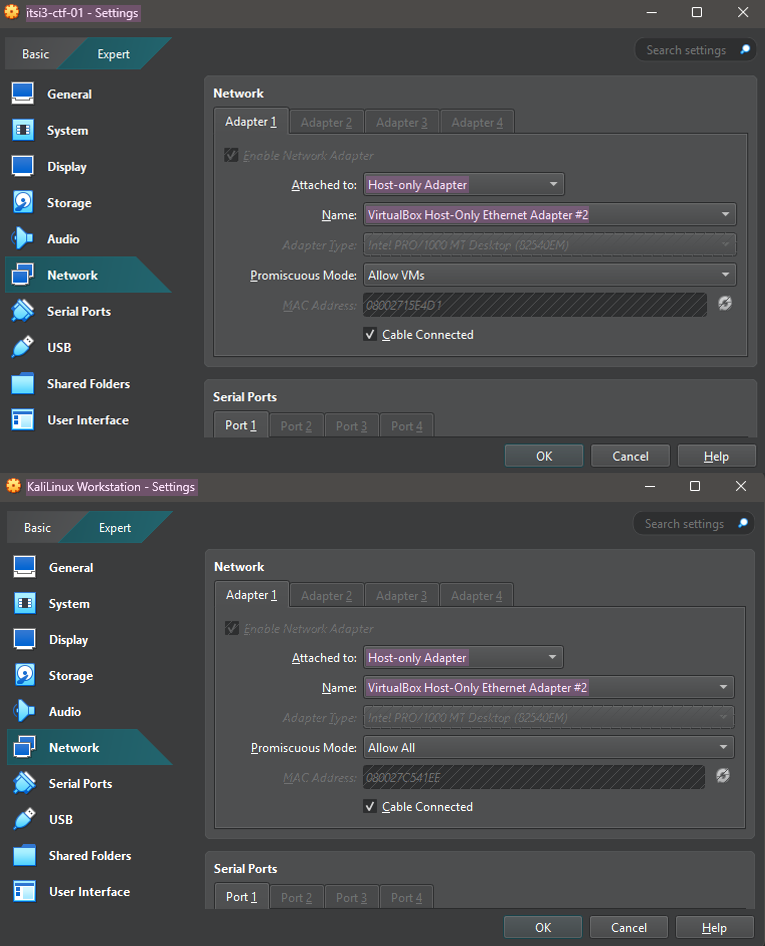
\includegraphics[scale=0.4]{./images/vmnwconf.png}
	\centering
	\caption{Showing the network configuration of the virtual machines}
\end{figure}\abc
\newpage
\subsection{Reconnaissance: Scanning the Network}
We use the Cyber Kill Chain to structure our steps for completing the CTF, with any attack beginning with reconnaissance, which in this case means scanning the network with \texttt{nmap}. Since we don't know the IP address of the target server yet, we need to scan the network to find it. For this, the command \texttt{nmap 192.168.15.0/24} is used to scan the entire network for open ports, as illustrated in Figure 6.\cite{cyberkillchain}
\begin{figure}[ht]
	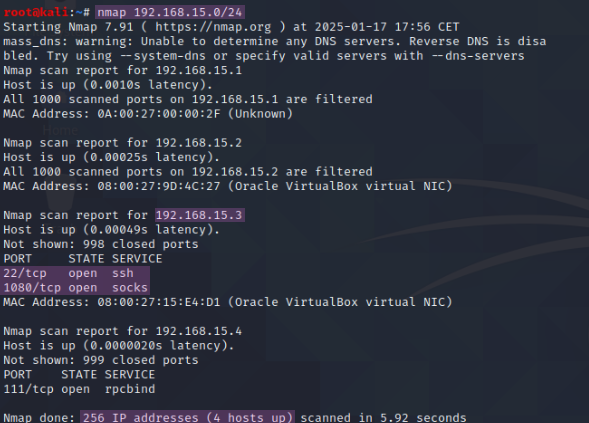
\includegraphics[scale=0.4]{images/firstnmapscan.png}
	\centering
	\caption{Results of the nmap scan}
\end{figure}\abc
We can determine that the target has the IP address \texttt{192.168.15.3}, since, as seen in \textcolor{blue}{\hyperref[fig:nwconf]{Figure \ref{fig:nwconf}}}, \texttt{.1} is the network address, \texttt{.2} is the \texttt{DHCP} server, and \texttt{.4} is the IP address of the Kali VM. This can be verified by running \texttt{ip a} or by scanning the open ports, since \texttt{ssh} is not exposed.
Now we can run another \texttt{nmap} scan to get fruther information abt the running servives and their version by using the \texttt{sV} flag and use the \texttt{T4} flag which sets the timing to agressive with the value 4 and the \texttt{p} falg with \texttt{-} value to scan all ports. The results of the scan can be seen in Figure 7.\cite{nmap-sv,nmap-t-flag}
\begin{figure}[h]
	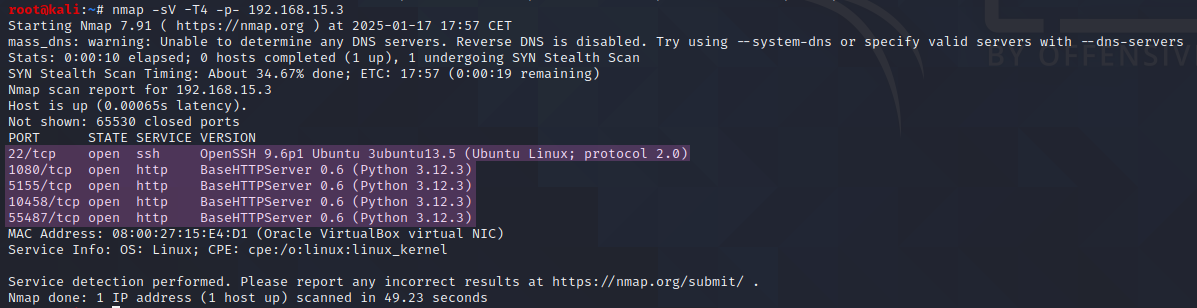
\includegraphics[scale=0.4]{images/nmapfr.png}
	\centering
	\caption{Results of the detailed nmap scan}
\end{figure}\abc
From this scan, we can see that \texttt{ssh} and four \texttt{http} servers running \texttt{Python 3.12.3} are active on the system.
\subsection{Reconnaissance: Exploring the websites}
If we open the websites in our web browser of choice, we can see that the one on port \texttt{1080} says that to get further, we need to scan deeper, which we already did. The website on port \texttt{5155} shows text from foreign languages, which is randomized and always prints out different text on refresh. The site on port \texttt{10458} prints out a message in \texttt{base64}, and lastly, the one on port \texttt{10448} has a basic authentication login prompt for a mini web shell. Figures 8 shows the content of each webpage.
\newpage
\begin{figure}[h]
	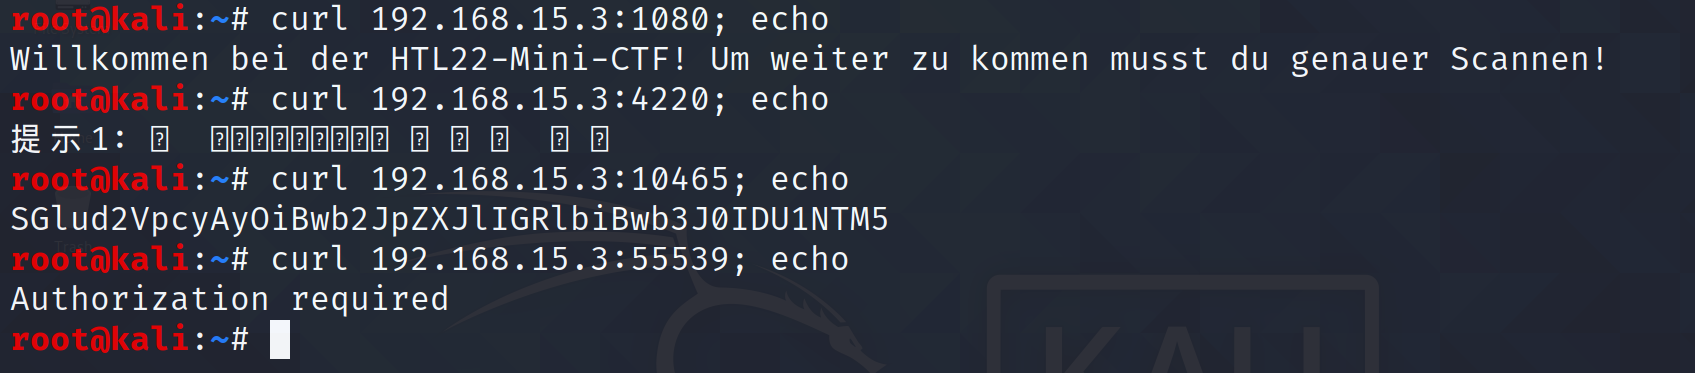
\includegraphics[scale=0.25]{images/allesiten.png}
	\centering
	\caption[a]{Showing the contents of each page using \texttt{curl} \footnotemark}
\end{figure}\abc
\footnotetext{The ports are different from those mentioned before, since instead of using screenshots from the browser, we opted to use \texttt{curl}. Additionally, on every refresh, the ports are randomized.}
The \texttt{base64} message can be decoded by piping the string, using \texttt{echo}, into the \texttt{base64} command, which gives us the hint to use port \texttt{55487}, the site with authentication. This is shown in Figure 9 below.
\begin{figure}[h]
	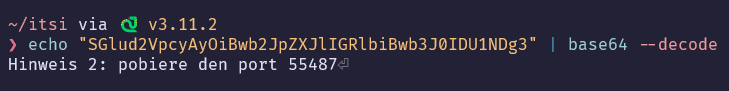
\includegraphics[scale=0.4]{images/base64.png}
	\centering
	\caption{Decoding the \texttt{base64} message}
\end{figure}\abc
To get all the random variants from the site with the foreign languages, I wrote a quick batch script to recursively relay the website and save the output in a file called \texttt{output}, as shown in Figure 10.
\begin{lstlisting}[language=bash]
#!/bin/bash
while true;do
    body=$(curl -s 192.168.15:5155)
    echo "$body" >> output
    echo "$body"
done
\end{lstlisting}
\begin{figure}[h]
	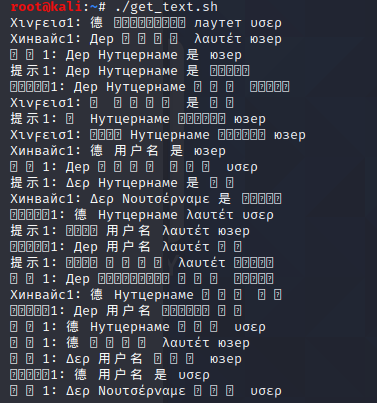
\includegraphics[scale=0.4]{images/gettextsh.png}
	\centering
	\caption{Running the script}
\end{figure}\abc
After running it for a while, we prompted ChatGPT with the list of outputs to translate, which revealed the following hint, as shown in Figure 11.
\begin{figure}[ht]
	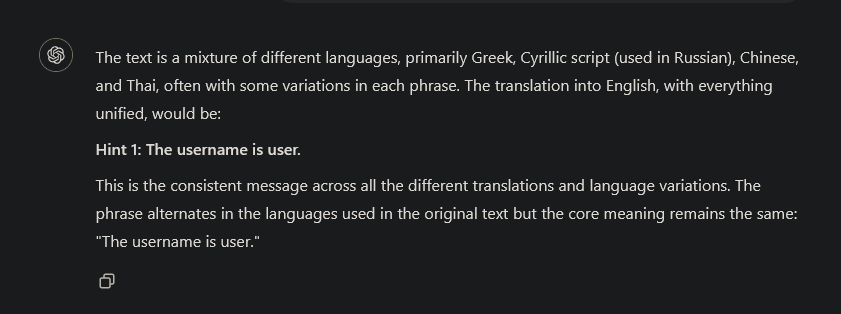
\includegraphics[scale=0.4]{images/labngs.png}
	\centering
	\caption{ChatGPT translating the hint}
\end{figure}\abc
\subsection{Weaponization: Evaluating the needed tools}
Now that we know the username and that it uses HTTP Basic Authentication, we can use Hydra to brute-force the password. For this, I have chosen the 10-million-password list as our wordlist \cite{pw-list}
\subsection{Exploitation: Using Hydra to break HTTP basic authentication}
To brute force the password, the following \texttt{hydra} command will be used: \texttt{hydra -l user -P pw.txt -s 55487 -f 192.168.15.3 http-get /}
Here is a breakdown of the options used in the command:\cite{hydra-http-basic-auth}
\begin{lstlisting}[language=bash]
-l user #specifying the username to attempt logging in with
-P pw.txt #tells Hydra to use the contents of pw.txt as passwords to try
-s 55487 #specifying the port to connect to
-f #telling Hydra to stop after a valid login
192.168.15.3 #setting the target IP address
http-get / #specifying the service and method to use
\end{lstlisting}
After running this command, we find out that the username is \texttt{user} and the password is \texttt{pass}, as seen in Figure 12.
\begin{figure}[h]
	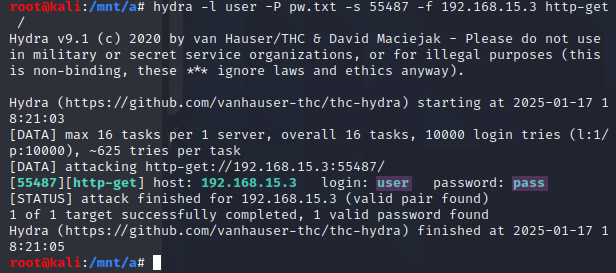
\includegraphics[scale=0.5]{images/hydra.png}
	\centering
	\caption{Running the Hydra command to get the credentials}
\end{figure}\abc
\newpage
After entering the found credentials on the webpage, we get the first flag.
\begin{figure}[h]
	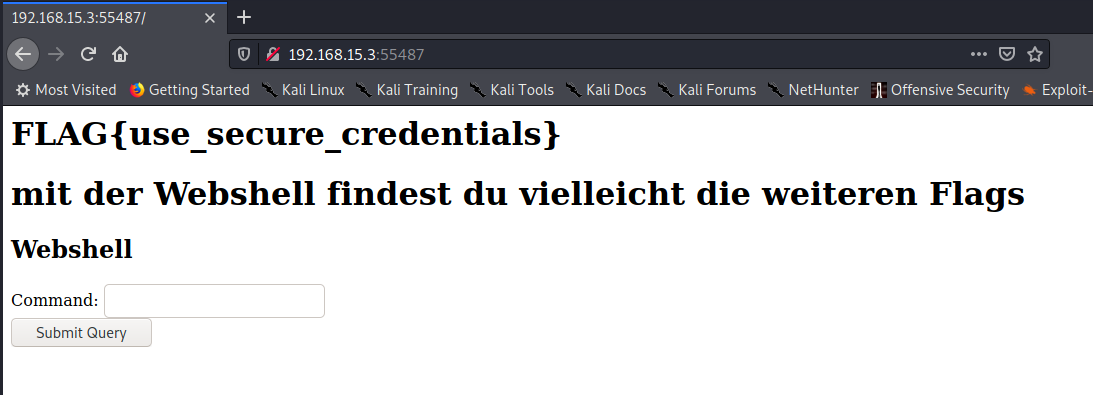
\includegraphics[scale=0.3]{images/flag1.png}
	\centering
	\caption{First flag found}
\end{figure}\abc
Besides the flag, there is a webshell on the site, so we can run commands on the server.
\subsection{sshing into the server}
\subsection{exploring the system}
\subsection{procces flag}
\subsection{comment flag}
\subsection{sudo flag}
\subsection{history flag}
\subsection{tmp flag}
\subsection{it's over but actually not}
\subsection{trying to escalate privaledgs}
\subsubsection{smart enumeration}
\subsubsection{trying a kernel level exploit}
\subsubsection{checking suid binarys}
\subsubsection{checking root proccses}
\subsubsection{trying metasploit}
\subsubsection{trying other common ctf priv escalation ways}
\subsection{reseting the root password and exploring the vm}
\subsection{7 flags}
\subsection{talking abt the setup etc or sum idk :shruge:}

\newpage
\section{References}
\bibliography{IEEEabrv,quellen}
\newpage
\section{List of figures}

\listoffigures

\end{document}
